 \section{Background}
Control Systems broadly come in two flavours: \textit{Open-loop} systems and \textit{Closed-loop} systems. Open-loop systems are systems which take in an input and execute it as perfectly as possible without any capability of inferring if the execution went as intended. The primary drawback of open-loop system is that it requires a perfect mathematical model of the complete system and its surrounding environment. Thus, open-loop systems work only in simple cases where it is easy to model all the factors that affect the output of the control system. In practice however, this is rarely the case. As a result, engineers have turned to closed-loop systems which have a feedback element that is used to minimize the error between the desired mission and the actual mission being executed. This is necessary since it is impossible to perfectly model beforehand the vagaries of the external disturbances as well as the noise inherent in the system.

Figure \ref{fig:control system} shows the representation of a closed-loop system. As described in the figure, a general closed-loop system has 4 components:


\begin{figure}
    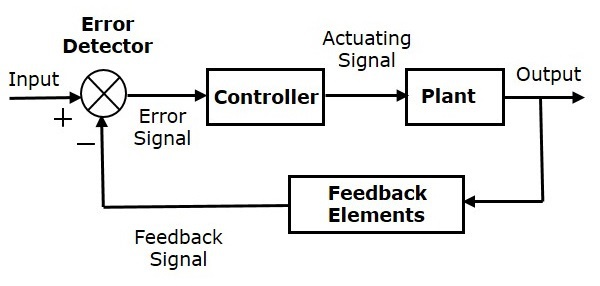
\includegraphics[scale=0.40]{images/closed_loop.jpg}
    \caption{Schematic diagram of a closed-loop control system. The feedback element which is used to correct the errors between the target output (which is a function of the input executed in ideal circumstances without noise and disturbances) and the observed output. The controllers are typically devices such as PLCs or microcontrollers running firmware.}
    \label{fig:control system}
\end{figure}


\begin{itemize}
    \item \textit{Controller:} Controller is a component that takes in the sensor values and converts it into control commands $z_k$ that is to be sent to the actuators. For example, the controller could be a PID controller that estimates and keeps track of position. We could have similar controller to provide feedback-based control to attitude(roll, pitch and yaw) of a UAV.
	\item \textit{Plant or Process:} The physical phenomena of interest, called the physical environment. For example, the position of a UAV or the acceleration of a UAV. The controller's task is to moderate the plant and steer it to the desired output. The controller accomplishes this using actuators. Actuators are components that executes the control commands sent by the controller. Typically, actuators are components such as motors and propellers that causes a change in physical environment around the CPS.
	\item \textit{Feedback Elements:} These are components which sense the outputs driven by the controllers and transmits it in a time-series, denoting the measurement of physical environment at every time instance. For example, the GPS sensor or accelerometer in a UAV is a sensor that sends in time series of position values to the controller.
 

\end{itemize}

\textbf{Cyber-Physical Systems(CPS)} CPS's are examples of closed loop systems, since, the physical subsystem executes commands from the computing system and the the computing subsystem consumes the sensor values perceived by the physical subsystem. Typically a physical subsystem consists of a combination of sensors and actuators. These two subsystems are connecting to form a feedback-based control system as shown in Figure \ref{fig:cps}

\begin{figure}
    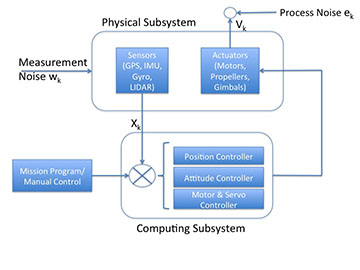
\includegraphics[scale=0.60]{images/cps-fig-small.jpg}
    \caption{Schematic diagram of a Cyber-Physical System, showing the Cyber and Physical realms in action. The diagram also shows the two kinds of noise in play in the physical world -- noise in measurement and noise in environment. These cause imperfect sensing and imperfect actuation repectively..}
    \label{fig:cps}
\end{figure}
%Insert picture of a cyber-physical system here with both cyber and physical aspects

As Figure \ref{fig:cps} describes, there are cyber and physical realms that are feedback control with one another. The mission control program could be as simple as preset waypoints on a map or it could be as complex as a neural network taking multiple inputs. In the case of a UAV, it could be something external such as manual commands using radio controller joystick to drive the UAV.  There are two kinds of noise that are in play here. First is the measurement noise, which gets mixed with the sensors while a measurement of the physical environment is obtained. In short, this noise accounts for imperfection in measurements and is typical in all measurement-based systems. Second is the process noise, which gets mixed with the environment when the controller drives the outputs to physical environment. In other words, this noise accounts for imperfect actuation.

\subsection{Attacks on CPS Systems}
There are multiple ways to compromise a CPS system. However, we would be generalizing the attacks into three broad categories. First, the attack could be on one of the actuators. This is typically done by intercepting the control command executed by the actuator to effect the physical environment around the CPS. In other words, the control command executed differs wildly from $v_k + e_k$ as it should be from Figure \ref{fig:cps}. This could result from the actuation mechanism itself being compromised or by accepting a control command from an untrusted agent. This false actuation will affect the measured variables of the physical environment and thereby the sensor measurements are also tampered.

Second, the attack could be on the sensors in the system. This is typically done by altering the perception of the physical environment around the CPS system. As a result, the sensor measurement used by the controller would be different from the real state of the measured variables. In other words, the physical process being measured differs wildly from $x_k + w_k$. Similar to attacks on actuators, attacks on sensors have the effect of circulating in the closed loop system, once injected.

Third, and perhaps the most grievous, is the case of the controller device getting compromised as well, giving the attacker unlimited control to implement any outcome. To detect this, one would need an unbiased view of the CPS system from an external vantage point that could be a trusted ground control station or a trusted UAV to perceive the state and compare it with the monitored UAV. 

In this paper, we are primarily concerned with attacks of the first two types of attacks -- attacks on actuators and sensors. We would be focusing on the design on a control-invariant framework that can help detect the attacks described. At a high level, our framework takes in measurements, say from sensors, $x_k$ and control commands, $V_k$  that are pushed out by the controller to the actuator and makes a binary decision of an attack via an anomaly detection technique. It is important to note that the idea of monitoring sensor measurements and control commands to identify issues with sensors, actuators or controllers is not a novel idea and is a popular idea in fault detection research. However, this style of fault detection relies on physical as well as spatial diversity (the technique of having multiple sensors or controllers and decide on majority voting) or functional redundancy(eg., measure a quantity directly as well as indirectly -- such as position being measured by double integrating acceleration). Furthermore, this sort of detection is not sufficient for an attacker, since, the effort to compromise multiple sensors having one compromised is O(1) -- via attack reuse. These attacks are shown in Fig \ref{fig:cps-attacks}. 

\begin{figure}
    \centering
    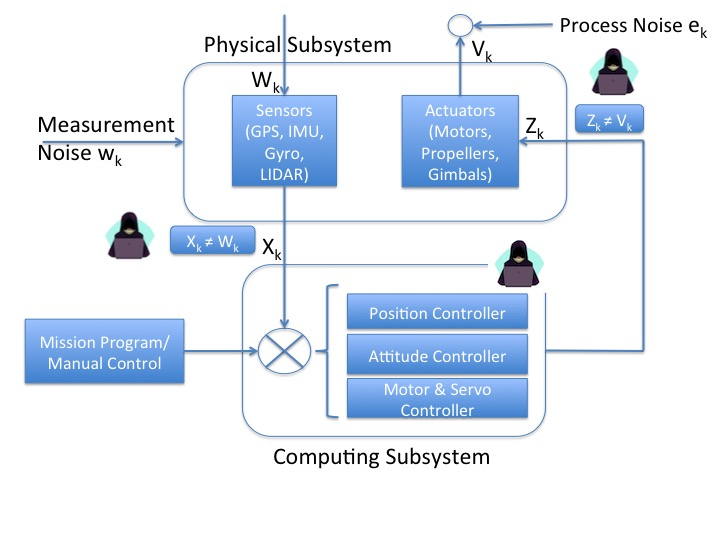
\includegraphics[scale=0.33]{images/cps-attacks.jpg}
    \caption{Attacks on a CPS system. The attacks can be on three regions -- sensors, actuators or the controller. The sensors and actuators form the physical subsystem and the controller which does the computing forms the compute subsystem of the CPS. In this paper, we are concerned only about the physical subsystem. The compute subsystem can be secured by using good security practices such as Control Flow Integrity \cite{abadi2005control}. }
    \label{fig:cps-attacks}
\end{figure}

\begin{figure*}
    \centering
    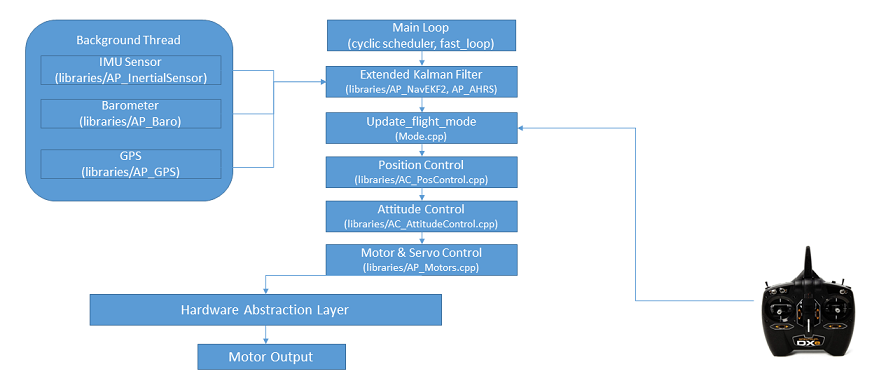
\includegraphics[width=\textwidth]{images/ardupilot-small.png}
    \caption{Architecture of an Autopilot. The main loop is run by a cyclic scheduler which polls sensor values periodically. The sensor values are fed into an Extended Kalman Filter which is used to estimate(correct) the sensor values and send it to position and attitute control layers. These are implemented as PID controllers which calculate the control signal that needs to be sent to the motors to perform the required navigation}
    \label{fig:ardupilot}
\end{figure*}

\subsection{Threat Model} The adversary is assumed to attack the physical components of the UAV viz., the sensors and/or actuators. The mode the adversary takes to accomplish this is irrelevant to our problem. Additionally, the adversary is assumed to not possess a knowledge of one of the following: 1) The Low-level parameters used in the controller, 2) The Physical model of the UAV. Lastly, we will assume that the UAV is not compromised via the computing subsystem and the compute subsystem is assumed to be secure.

\subsection{Software Architecture of a UAV System} UAVs need a navigation software to make it \textit{unmanned} as opposed to just receiving commands from a radio transceiver and navigate accordingly. This software performs the navigation by computation based on reading sensor values and  Ardupilot is an open-source autopilot software that is capable of controlling autonomous drones, helicopters, boats, submarines, and antenna trackers. The ardupilot software suite consists of navigation software, called firmware when it is compiled into a binary for microcontroller-based hardware hosts \cite{anderson2016ardupilot, wiki:xxx}.

As seen in the Figure \ref{fig:ardupilot}, Ardupilot software stack consists of a cyclic scheduler that triggers a main loop at periodic intervals. The main loop consists of a polling of GPS and IMU sensors which give the position and attitude of the UAV. The GPS sensors give an estimate of the linear position by means of latitude and longitude values. The IMU is a unit consisting of accelerometer, gyroscope, and magnetometer. Typically, there is one accelerometer,gyroscope and magnetometer per axis for each of the three vehicle axes: pitch, roll and yaw. The three vehicle axes are shown in Figure \ref{fig:imu}. It is shown in CPS and optimal control theory research \cite{dissanayake2001solution} that using these sensors in isolation leads to drift and estimation errors. As a result, these values are passed onto an Extended Kalman Filter(EKF) which is used to correct these errors and provide \textit{optimal estimation} for sensors in the presence of noise. Let us consider the example of position and attitude estimate, which is the problem of estimating the coordinates of x, y and z along with their angular versions (roll, pitch and yaw). EKF achieves this by fusing the values from IMU and GPS in conjunction with its knowledge of estimated noise in each of the measurement channels. Note that this approach of correcting sensory measurements can equally be applied for other sensors such as barometer (pressure) or wind sensor as well though those are less interesting from a security standpoint \cite{raginskyuiuc}.

\subsubsection{The Extended Kalman Filter} The following steps are a highly non-mathematical gist of how the Extended Kalman Filter(EKF) works in practice:

\begin{enumerate}
    \item IMU angular acceleration values are double integrated to derive angular position values
    \item The IMU angular position vales are converted from the frame of the UAV to the frame of earth. Using this, a corrected value of IMU angular acceleration value is calculated.
        \begin{itemize}
            \item This is done since GPS values are along the earth's coordinate system but IMU values are along the UAV's roll, pitch, yaw coordinate system. 
        \end{itemize}
        
    \item The corrected IMU accelerations are single integrated to derive velocity estimates
    \item The IMU velocity estimates are single integrated to derive position estimates.

\noindent Steps 1 to 4 collectively is known as the  \textit{State Prediction} process. State is a variable that is to be estimated such as roll, pitch, yaw.
    
    \item The IMU keeps an estimate of accelerometer noise. This is used to estimate the growth in errors in position, velocity and their angular counterparts. These errors are captured in a large matrix called the \textit{State Covariance Matrix}.
    
\noindent Note that until now, GPS values are not used. Now suppose a GPS measurement comes in.

    \item The GPS measurement is used to calculate the difference between position calculated in Step 4 and the GPS measurement. This value is called \textit{innovation}
    
    \item The innovation value, state covariance matrix is combined with the GPS noise estimate (similar to the IMU accelerometer noise) to obtain a correction in position, velocity and their angular counterparts.
    
    \item The state covariance matrix used in step 5 is updated and the process is repeated.

\end{enumerate}
 
\subsubsection{The SLAM problem} Simultaneous Localization and Mapping, better known as SLAM, is an algorithms used in robotics. This is common when a UAV enters a hitherto unknown environment having  to perform spatial exploration and navigate accordingly. The SLAM problem is solved by using a Extended Kalman Filter, which has the capability to optimally estimate the state of a UAV in presence of noise. Again keeping the discussion highly non-mathematical, SLAM solution consists of 3 operations, iterated at every single time-step: \cite{bailey2006consistency}

\begin{enumerate}
    \item The UAV moves, reaching a new point of the scene. Due to unavoidable noise and errors, this motion increases the uncertainty in the position values of the UAV.
    
    \item The UAV discovers interesting features in the environment, which need to be incorporation into the map. This step is called Mapping and the features are called landmarks. Due to errors in the sensors, the location of these landmarks is uncertain. This is in conjunction with the uncertainty in the position values of the UAV. Thus, there are 2 uncertainties at this stage.
    
    \item The UAV observes landmarks that has been previously mapped. This is used to correct the position of landmarks and the UAV's position. Thus, after this step, the position uncertainty of the UAV and position uncertainty of the landmark are corrected.
\end{enumerate}

These values obtained in this three steps are fed into an Extended Kalman Filter(EKF) to correct the errors and build an automated solution for navigation.

